\section{Inferential Statistic}
\tab We plan to construct a Multiple Linear Regression (MLR) model where Memory\_Speed serves as the output or dependent variable. The independent variables, including Memory, Memory\_Bandwidth, Core\_Speed, Memory\_Bus, Memory\_Type, Process, Texture\_Rate, and Pixel\_Rate, will be utilized. Our aim is to predict the missing values of Memory\_Speed in the original dataset using the MLR model, while also examining the relationship between Memory\_Speed and the independent variables. Following the assessment of MLR assumptions, aside from normality, we proceed with splitting the dataset and constructing the model.

\subsection{Sample splitting}
\tab We partitioned the dataset into training and testing subsets to ensure accurate model evaluation. Initially, the model is trained using the training data, followed by refinement using the test data. It's essential to note that evaluating the model solely on the training data is insufficient as it may not generalize well to unseen data.  

\tab For this project, we opted for an 80/20 ratio of training to testing data. 

\begin{center}
    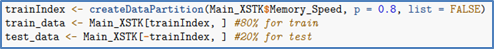
\includegraphics[width=0.8\textwidth]{Sample-splitting.png}
\end{center}

\subsection{Importance of variables}
\tab Higher the value of mean decrease accuracy or mean decrease gini score, higher the importance of the variable in the model. In the plot shown above, Memory\_Bandwidth is most important variable. 

\begin{center}
    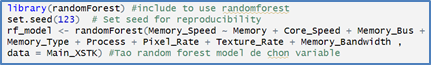
\includegraphics[width=0.8\textwidth]{importance.png}
\end{center}

\begin{center}
    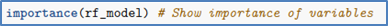
\includegraphics[width=0.8\textwidth]{importance1.png}
\end{center}

\begin{center}
    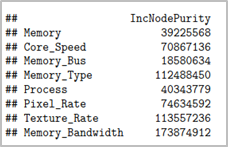
\includegraphics[width=0.7\textwidth]{importance2.png}
\end{center}

\begin{center}
    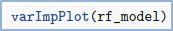
\includegraphics[width=0.4\textwidth]{importance3.png}
\end{center}

\begin{center}
    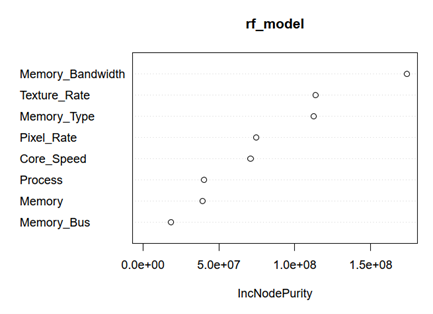
\includegraphics[width=0.8\textwidth]{importance4.png}
\end{center}

\subsection{Building multiple linear regression model}

\begin{center}
    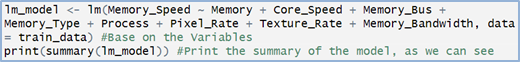
\includegraphics[width=0.8\textwidth]{Build-model.png}
\end{center}

\begin{center}
    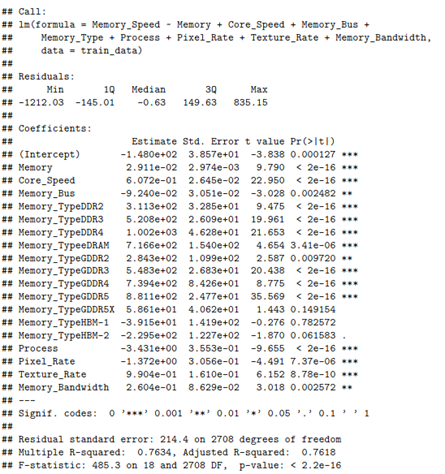
\includegraphics[width=0.8\textwidth]{Build-model1.png}
\end{center}

\tab The variables Memory\_TypeGDDR5X, Memory\_TypeHBM-1, and 
Memory\_TypeHBM-2 are not statistically significant as their p-values are much greater than 0.05. This indicates that these variables do not make a significant contribution to the model and can be removed. Residual standard error stands at 214.4, indicating that actual GPU prices may deviate from the true regression line by roughly 214.4 USD. 

\tab Adjusted R-squared value of 0.7634 indicates that approximately 76.34\% of the variability in the data can be explained by the model. In this case, with an F-statistic of 485.3 and a p-value below 0.05, we can confidently reject the null hypothesis. This means that there is strong evidence to suggest that at least one of the independent variables included in the model is related to the dependent variable (Memory\_Speed). Therefore, we have reason to believe that there is a relationship between the independent variables and the dependent variable.

\subsection{Test for assumptions}
\subsubsection{Assumption 1: Linearity of the Data}
\tab We can check the linearity of the data by looking at the Residual versus Fitted plot. 

\begin{center}
    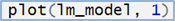
\includegraphics[width=0.4\textwidth]{test-ass1.1.png}
\end{center}

\begin{center}
    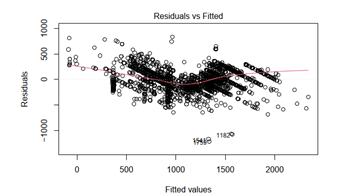
\includegraphics[width=0.8\textwidth]{test-ass1.2.png}
\end{center}
\tab  This red line is not too straight on the 0 line, but it's still acceptable for this model.

\subsubsection{Assumption 2: Predictors (x) are Independent \& Observed with Negligible Error}

\tab The easiest way to check the assumption of independence is using the Durbin-Watson test. 

\begin{center}
    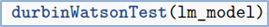
\includegraphics[width=0.4\textwidth]{test-ass2.1.png}
\end{center}

\begin{center}
    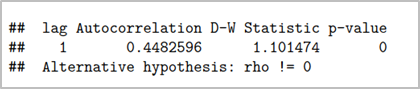
\includegraphics[width=0.8\textwidth]{test-ass2.2.png}
\end{center}

\tab The null hypothesis states that the errors are not auto-correlated with themselves (they are independent). Thus, if we achieve a $p-value >$ 0.05, we would fail to reject the null hypothesis. This would give us enough evidence to state that our independence assumption is met!

\subsubsection{Assumption 3: Residual Errors have a Mean Value of Zero}

\begin{center}
    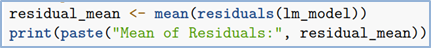
\includegraphics[width=0.8\textwidth]{test-ass3.1.png}
\end{center}

\begin{center}
    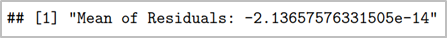
\includegraphics[width=0.8\textwidth]{test-ass3.2.png}
\end{center}

\tab  This value is $-2.14\cdot 10^{-14}$, approximate 0, so this assumption has been met. 

\subsubsection{Assumption 4: Residual Errors have Constant Variance}

\begin{center}
    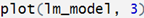
\includegraphics[width=0.4\textwidth]{test-ass4.1.png}
\end{center}

\begin{center}
    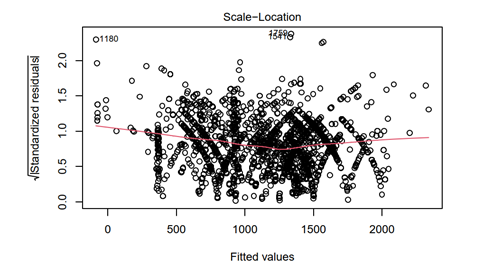
\includegraphics[width=0.8\textwidth]{test-ass4.2.png}
\end{center}

\tab Ideally, we would want to see the residual points equally spread around the red line, which would indicate constant variance. However, it is acceptable. 

\subsubsection{Assumption 5: Testing for normality of the errors}

\tab To check this, we have to use $Q-Q$ plot for normality consideration. The output we expect that the residuals will mostly scatter close to the straight line to get normality hypothesis accepted. 

\begin{center}
    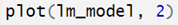
\includegraphics[width=0.4\textwidth]{test-ass5.1.png}
\end{center}

\begin{center}
    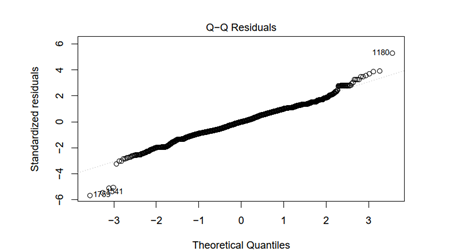
\includegraphics[width=0.8\textwidth]{test-ass5.2.png}
\end{center}

\tab We can conclude that this model can be normally accurate, not 100\% accurate. Perhaps another model will be more fitted for this data. 

\subsubsection{Testing for accuracy}

\begin{center}
    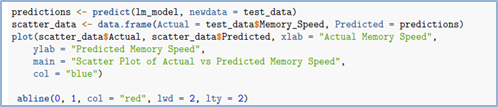
\includegraphics[width=0.8\textwidth]{test-accuracy1.png}
\end{center}

\tab In an ideal scenario, where the predicted memory speeds perfectly match the actual memory speeds, all the points would fall on a diagonal line with a slope of 1 (y = x). Deviations from this diagonal line indicate discrepancies between the actual and predicted values.  

\begin{center}
    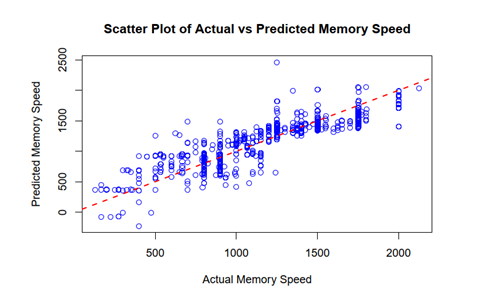
\includegraphics[width=0.8\textwidth]{test-accuracy2.png}
\end{center}

\begin{center}
    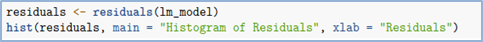
\includegraphics[width=0.8\textwidth]{test-accuracy3.png}
\end{center}

\begin{center}
    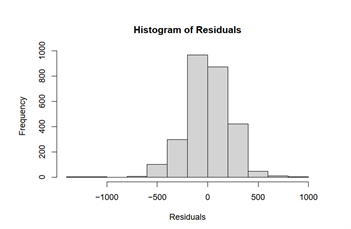
\includegraphics[width=0.8\textwidth]{test-accuracy4.png}
\end{center}

\tab  By examining the histogram of residuals, you can assess 
whether the residuals are approximately normally distributed, 
which is an assumption of many linear regression models. If the histogram shows a roughly bell-shaped curve, it suggests that the assumption is reasonable.  

\begin{center}
    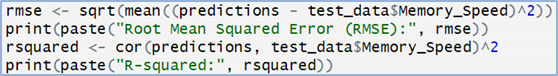
\includegraphics[width=0.8\textwidth]{test-accuracy5.png}
\end{center}

\begin{center}
    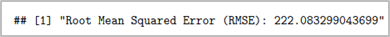
\includegraphics[width=0.8\textwidth]{test-accuracy6.png}
\end{center}

\begin{center}
    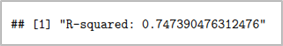
\includegraphics[width=0.8\textwidth]{test-accuracy7.png}
\end{center}

\tab This dataset is ranged from 10 to ~1700 so this error can be assume as small value so it can be accepted. 

\begin{center}
    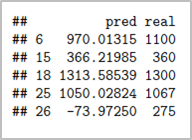
\includegraphics[width=0.5\textwidth]{test-accuracy8.png}
\end{center}

\begin{center}
    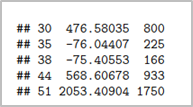
\includegraphics[width=0.5\textwidth]{test-accuracy9.png}
\end{center}

\subsection{Building random forest model}

\begin{center}
    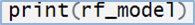
\includegraphics[width=0.3\textwidth]{build-forest1.png}
\end{center}

\begin{center}
    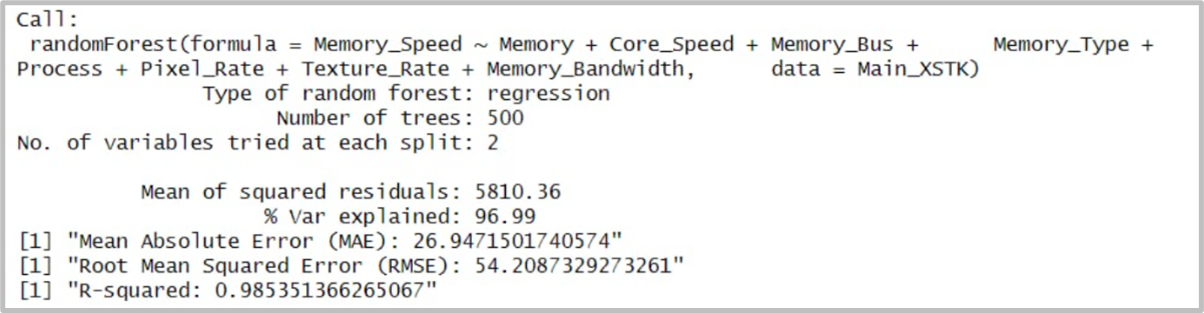
\includegraphics[width=0.8\textwidth]{build-forest2.png}
\end{center}

\tab where:
\begin{itemize}
    \item \textbf{Type of Random Forest:} Indicates whether the Random Forest model is used for regression or classification. In this case, it is a regression Random Forest, meaning it is used for predicting numeric values (Memory\_Speed). 
    \item \textbf{Number of Trees:} Specifies the number of decision trees created by the Random Forest algorithm. Random Forest builds multiple decision trees and combines their predictions to improve the accuracy and robustness of the model. In this example, the model consists of 500 decision trees.
    \item \textbf{No. of Variables Tried at Each Split:} Indicates the number of predictor variables considered for each split in the decision trees. Random Forest randomly selects a subset of predictor variables at each split to create diverse trees. In this example, 4 predictor variables are tried at each split.
    \item \textbf{Mean of Squared Residuals:} The mean of the squared differences between the actual values and the predicted values (residuals) of the target variable (Memory\_Speed). It provides a measure of the model's accuracy. A lower value indicates better performance, as it means the model's predictions are closer to the actual values. (5810.36 is a really good outcome, better than linear regression(x2)). 
    \item \textbf{\%Var:} The percentage of variance explained by the mode, the higher the \%Var, the better the model.
    
\end{itemize}

\begin{center}
    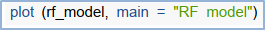
\includegraphics[width=0.4\textwidth]{build-forest3.png}
\end{center}

\begin{center}
    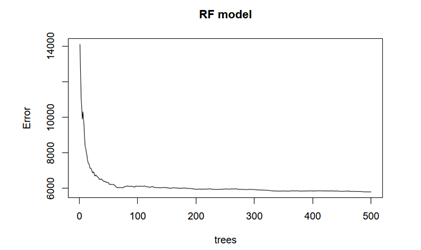
\includegraphics[width=0.8\textwidth]{build-forest4.png}
\end{center}

\subsubsection{Test for accuracy}

\begin{center}
    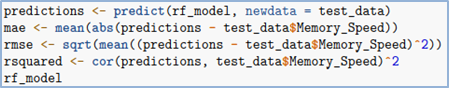
\includegraphics[width=0.8\textwidth]{test-forest1.png}
\end{center}

\begin{center}
    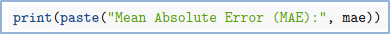
\includegraphics[width=0.8\textwidth]{test-forest2.png}
\end{center}

\begin{center}
    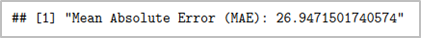
\includegraphics[width=0.8\textwidth]{test-forest3.png}
\end{center}

\begin{center}
    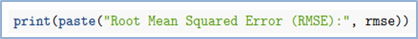
\includegraphics[width=0.8\textwidth]{test-forest4.png}
\end{center}

\begin{center}
    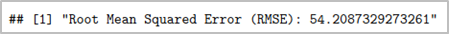
\includegraphics[width=0.8\textwidth]{test-forest5.png}
\end{center}

\begin{center}
    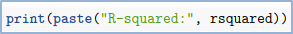
\includegraphics[width=0.8\textwidth]{test-forest6.png}
\end{center}

\begin{center}
    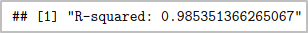
\includegraphics[width=0.8\textwidth]{test-forest7.png}
\end{center}

\tab $\rightarrow$ This Value is really near 1, so this may be the most fit model for our dataset.

\begin{center}
    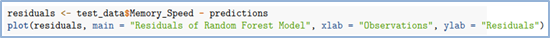
\includegraphics[width=0.8\textwidth]{test-forest8.png}
\end{center}

\begin{center}
    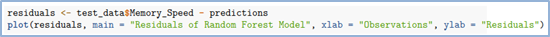
\includegraphics[width=0.8\textwidth]{test-forest9.png}
\end{center}

\begin{center}
    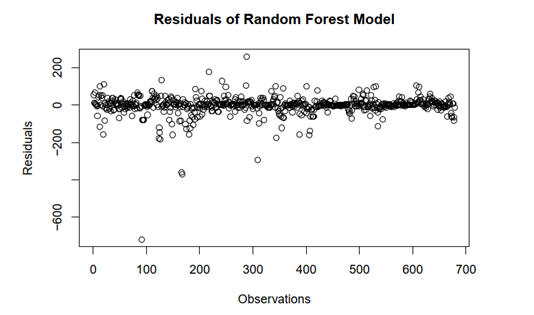
\includegraphics[width=0.8\textwidth]{test-forest10.png}
\end{center}

\tab $\rightarrow$ The ideally output is the distribution perfectly lines on the $x – axis$. Therefore, this output is acceptable. 

\begin{center}
    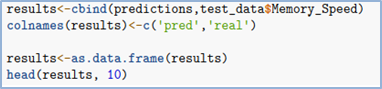
\includegraphics[width=0.6\textwidth]{test-forest11.png}
\end{center}

\begin{center}
    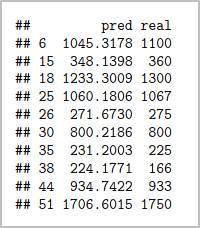
\includegraphics[width=0.5\textwidth]{test-forest12.png}
\end{center}